\documentclass[12pt,t]{beamer}
\usepackage{amsmath, graphicx, kbordermatrix,bm, animate,hyperref,color}


\usepackage{tikz}
\usetikzlibrary{positioning}

\setbeameroption{hide notes}
\setbeamertemplate{note page}[plain]



% page number
\setbeamertemplate{footline}{%
    \raisebox{5pt}{\makebox[\paperwidth]{\hfill\makebox[20pt]{\color{gray}
          \scriptsize\insertframenumber}}}\hspace*{5pt}}

% add a bit of space at the top of the notes page
\addtobeamertemplate{note page}{\setlength{\parskip}{12pt}}


% a few macros
\newcommand{\subt}[1]{{\footnotesize \color{subtitle} {#1}}}

% title info
\title{``Creative'' AI}
\author{\href{http://richcorrado.github.io}{Richard Corrado}}
\institute{Fat Cat Machine Learning}
\date{\href{https://github.com/richcorrado}{\tt \scriptsize github.com/richcorrado}}

\begin{document}

% title slide
{
	\setbeamertemplate{footline}{} % no page number here
	\frame{
		\titlepage
} } 
	


\begin{frame}{Goals}

\begin{itemize}
\item Review some general concepts of Machine Learning.
\item Motivate and review Neural Networks (NNs), including Convolutional and Recurrent NNs.
\item Survey applications of NNs to visual, audio, and textual media.
\item Objective is to transform an object or mimic a human task according to information learned from training examples, rather than classic ML goal of prediction.
\end{itemize}


\end{frame}

\begin{frame}{Classic Machine Learning}

From some quantities $\mathbf{x}$ (the {\bf features}), predict a value for a quantity $y$ (the {\bf target}).   In principle, there is some functional relationship
$$ y = f(\mathbf{x}).$$
However:
\begin{itemize}
\item Detailed form of $f$ is unknown (complexity of underlying system).
\item Predictors $\mathbf{x}$ may be incomplete or imperfect (complexity of data, randomness). Even if we knew $f$,  could only compute within some margin of error
$$ f(\mathbf{x}) = y \pm \epsilon.$$
\end{itemize}

\end{frame}

\begin{frame}

{\bf Machine Learning} (ML)  includes the study and application of algorithmic models to find approximations  
$$ \hat{f}(\mathbf{x} )\approx f(\mathbf{x}). $$
Statistical principles of validation, inference, etc., are used to determine the errors of the models.


\bigskip

{\bf Regression}: Target $y$ is a continuous variable.
\begin{itemize}
\item Prices or other expected values. 
\item Expected demand in number of units  (approximately continuous for large numbers).
\item Physical dimension of object (area, mass).
\end{itemize}

\end{frame}

\begin{frame}

{\bf Classification}: Target $y$ takes some discrete and finite number of values.

\begin{itemize}
\item What is the species of the object? (Iris classification)
\centerline{
\includegraphics[height=0.5\textheight]{./images/iris.png}
}  
\end{itemize}

\end{frame}

\begin{frame}
\begin{itemize}
\item Image recognition
\centerline{
\includegraphics[height=0.8\textheight]{./images/dogorbear.png}
} 
\end{itemize}

\end{frame}


\begin{frame}{Neural Networks}


In order to keep the training process mathematically stable and computationally managable, NNs are based on fairly simple functions:
\begin{itemize}
\item Linear functions:
\begin{equation*} \begin{split}
&  \mathbf{z^{(i)}} = \mathbf{f}^{(i-1)} \mathbf{W}^{(i)} + \mathbf{b}^{(i)}, \\
&  \mathbf{W}^{(i)}: ~~\text{weights, with shape}~(F_{i-1}, F_i), \\
&   \mathbf{b}^{(i)}:~~~~\text{biases, with shape}~( F_i).
\end{split} \end{equation*}
\item Nonlinear functions, called {\bf activation functions}:
$$ \mathbf{f}^{(i)} = g^{(i)}(\mathbf{z}^{(i)}).$$
\item So each layer learns {\bf new features}:
$$ \mathbf{f}^{(i)} = g^{(i)} \Bigl(\mathbf{f}^{(i-1)} \mathbf{W}^{(i)} + \mathbf{b}^{(i)}\Bigr).$$
\end{itemize}
\end{frame}

\begin{frame}

Terminology for the layers is:
\begin{itemize}
\item {\bf Input layer}: The first layer of the network is designed to simply load in the input features $\mathbf{x}$ present in the dataset.
\item {\bf Output layer}: The last layer is designed to produce an output that can be compared directly to the targets $\mathbf{y}$.
\item {\bf Hidden layers}: The layers in between compute the new features $\mathbf{f}^{(i)}$.  Not connected to input or output. 
\item {\bf Width}: Number of new features of a single hidden layer. 
\item {\bf Depth}: Total number of hidden layers in the network.  If depth is $\geq 3$ we can say that we have a {\bf deep neural network}.
\end{itemize}
\end{frame}


\begin{frame}{Single Hidden Layer}


\tikzset{%
  every neuron/.style={
    circle,
    draw,
    minimum size=1cm
  },
  neuron missing/.style={
    draw=none, 
    scale=4,
    text height=0.333cm,
    execute at begin node=\color{black}$\vdots$
  },
}

\begin{center}
\resizebox{7.0cm}{!}{
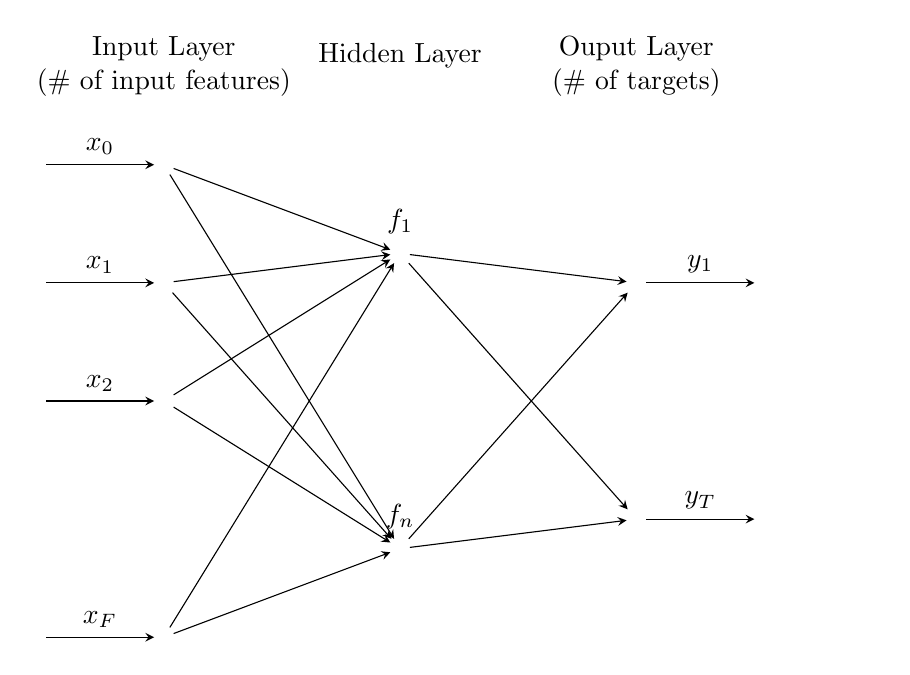
\begin{tikzpicture}[x=1.5cm, y=1.5cm, >=stealth]

\foreach \m/\l [count=\y] in {1,2,3,missing,4}
  \node [every neuron/.try, neuron \m/.try] (input-\m) at (0,2.5-\y) {};

\foreach \m [count=\y] in {1,missing,2}
  \node [every neuron/.try, neuron \m/.try ] (hidden-\m) at (2,2-\y*1.25) {};

\foreach \m [count=\y] in {1,missing,2}
  \node [every neuron/.try, neuron \m/.try ] (output-\m) at (4,1.5-\y) {};

\foreach \l [count=\i] in {0,1,2,F}
  \draw [<-] (input-\i) -- ++(-1,0)
    node [above, midway] {$x_\l$};

\foreach \l [count=\i] in {1,n}
  \node [above] at (hidden-\i.north) {$f_\l$};

\foreach \l [count=\i] in {1,T}
  \draw [->] (output-\i) -- ++(1,0)
    node [above, midway] {$y_\l$};

\foreach \i in {1,...,4}
  \foreach \j in {1,...,2}
    \draw [->] (input-\i) -- (hidden-\j);

\foreach \i in {1,...,2}
  \foreach \j in {1,...,2}
    \draw [->] (hidden-\i) -- (output-\j);

\foreach \l [count=\x from 0] in {Input Layer \\ (\# of input features), Hidden  Layer \\ \hfill, Ouput  Layer  \\ (\# of targets),}
  \node [align=center, above] at (\x*2,2) {\l };
\end{tikzpicture}
} \end{center}

A network like this, where every input feature is connected to a new feature is called a {\bf feedforward network} or, in older terms, a {\bf multilevel perceptron} (MLP).


\end{frame}

\begin{frame}{Composition of Functions}

Recall that a typical goal of machine learning is to approximate the functional relationship between the input features $\mathbf{x}$ and some target output $\mathbf{y}$:
$$ \mathbf{y} = f(\mathbf{x}) .$$
NNs naturally arrive at an approximation of this function via the composition of the functions learned at the hidden layers:
$$ \hat{f}(\mathbf{x}) = f^{(H)} \circ \cdots \circ f^{(1)}(\mathbf{x}).$$


\end{frame}


\begin{frame}{Modifications of Feedforward Architecture}
In a fully-connected feed-forward network, each hidden layer feature is connected to a feature from the previous layer
$$ z_{a_i}^{(i)} = \sum_{a_{i-1}=0}^{F_{i-1}-1} f^{(i-1)}_{a_{i-1}} W_{a_{i-1} a_i}^{(i)} + b_{a_i}^{(i)}. $$
We can modify the rules for computing the new features, creating new {\bf architectures}, new types of NNs.

\begin{itemize}
\item[1.] We can force some of the weights  $W^{(i)}_{a_{i-1}a_i}$ to zero.  This generally results in fully-connected models with a smaller capacity.
\centerline{
\includegraphics[height=0.2\textheight]{./images/dropout.png}
} 
\end{itemize}
\end{frame}

\begin{frame}
\begin{itemize}
\item[2.]  We can impose some symmetry on the weights $W^{(i)}_{a_{i-1}a_i}$, forcing some components to be equal to one another. This is called {\bf weight sharing}.
\item[3.] We can remove some connections to the previous layer. This is equivalent to replacing 
$$ \mathbf{f}^{(i-1)} \mathbf{W}^{(i)} \rightarrow \sum_{a_{i-1} \in D} f^{(i-1)}_{a_{i-1}} W^{(i)}_{a_{i-1}a_i},$$
where $D$ is some subset of the index set for the incoming features $\mathbf{f}^{(i-1)}$. 
\centerline{
\includegraphics[height=0.4\textheight]{./images/semiconnect.png}
} 
\end{itemize}
\end{frame}

\begin{frame}
\begin{itemize}
\item[4.]  Can have more general connections between layers.
\begin{itemize}
\item {\bf Recurrent} networks have a chain structure between layers.

\centerline{
\includegraphics[height=0.4\textheight]{./images/recurrent.png} 
}
\item {\bf Recursive} networks have a tree structure.

\bigskip

\centerline{
\includegraphics[height=0.2\textheight]{./images/recursive.png}
} 
\end{itemize}
\end{itemize}

\end{frame}

\begin{frame}{Convolutional Neural Networks}

Convolutional NNs (CNNs) are designed to preserve information about how pixels in 2D images are spatially related:
\centerline{
\includegraphics[height=0.4\textheight]{./images/convolution.png} 
}
\begin{itemize}
\item {\bf  Partial connectivity}: Sample nearby pixels using a window.
\item {\bf Weight sharing}: Weights are shared over the whole image. 
\end{itemize}
\end{frame}

\begin{frame}

{\bf Filter}: Collection of weights forming a window.  Can use different filters to compute multiple types of features for a given image:

\centerline{
\includegraphics[height=0.4\textheight]{./images/convolution2.png} 
}

{\bf Translational invariance}: CNN filters tend to learn geometric shapes, regardless of where they appear in an image:

\centerline{
\includegraphics[height=0.3\textheight]{./images/convfeat.png} 
}

\end{frame}

\begin{frame}{Computer Vision}

Since CNNs are well-suited for processing 2D images (but can also be used for 3D and non-image problems),  they are extensively used in machine learning with images.

\begin{itemize}
\item {\bf Character recognition}: MNIST digits, zip codes:

\centerline{
\href{http://yann.lecun.com/exdb/lenet/gifs/asamples.gif}{\includegraphics[height=0.3\textheight]{./images/lenet-22.png}}
}
%\animategraphics[loop,controls,width=0.8\linewidth]{12}{./images/lenet-}{0}{30}
\end{itemize}
\end{frame}

\begin{frame}

Google Streetview: {\bf localization} and character recognition

\centerline{
\includegraphics[height=0.8\textheight]{./images/streetview.png} 
}

\end{frame}

\begin{frame}

ImageNet: {\bf object detection}

\centerline{
\includegraphics[height=0.8\textheight]{./images/imagenet-objdet.png} 
}

\end{frame}

\begin{frame}

ImageNet: {\bf classification}

\centerline{
\includegraphics[height=0.8\textheight]{./images/imagenet.png} 
}

\end{frame}

\begin{frame}

ImageNet: classification + {\bf localization}

\centerline{
\includegraphics[height=0.5\textheight]{./images/LocalizationDetection.png} 
}

\end{frame}





\begin{frame}{VGG-Network}
\href{http://www.robots.ox.ac.uk/~vgg/research/very_deep/}{\color{blue} Simonyan and Zisserman},  ICLR 2015, 
\href{https://arxiv.org/abs/1409.1556}{\color{blue}arxiv:1409.1556},  1st/2nd in localization/classification, ImageNet ILSVRC-2014.

 \centerline{
\includegraphics[height=0.7\textheight]{./images/vgg19.png} 
}

\end{frame}

\begin{frame}{A Neural Algorithm of Artistic Style}
Gatys, Ecker,  Bethge,  Journal of Vision (2015), \href{https://arxiv.org/abs/1508.06576}{\color{blue}arxiv:1508.06576}.

\bigskip

Consider a CNN trained on object recognition:

\bigskip

{\bf Content representation}: At each layer, features capture the high-level {\bf content} (objects + arrangement), but not exact pixel values 

\bigskip

{\bf Style representation}: 
Study correlations between the features at a given layer  $\longrightarrow$ discards spatial information, but provides a stationary description of the texture of an image.  

\bigskip

{\bf Method}:  Learn style representation by mapping a white noise image onto the texture of the image.

\end{frame}

\begin{frame}
 \centerline{
\includegraphics[height=0.9\textheight]{./images/texture-analysis.png} 
}
\end{frame}

\begin{frame}{Details}
$F_{ij}^l$ is the activation of the $i^{th}$ filter at position $j$ in layer $l$. \\
$\vec{p}$: original image, ~~ $\vec{x}$: white-noise image \\
Cost function for content representation: 
\begin{equation*}
\mathcal{L}_{content}(\vec{p},\vec{x},l) = \frac{1}{2}\sum_{i,j}\left(F^l_{ij} - P^l_{ij}\right)^2 \text{ .}
\end{equation*}
Cost function for style representation: 
\begin{equation*}
\begin{split}
& \mathcal{L}_{style}(\vec{a},\vec{x}) = \sum_{l=0}^{L}w_{l}E_l, \\
& E_l = \frac{1}{4 N_l^2 M_l^2}\sum_{i,j}\left(G^l_{ij}-A^l_{ij}\right)^2, \\
& G_{ij}^l = \sum_k F_{ik}^l F_{jk}^l.
\end{split}
\end{equation*}

\end{frame}

\begin{frame}{Style Transfer}

Combine {\bf content representation} of one image with {\bf style representation} of another image.

\bigskip 

Suppose: 

\hspace{1cm} $\vec{p}$ is a photograph: the {\bf content}, \\
\hspace{1cm} $\vec{a}$ is an artwork with a distinct textural {\bf style}\\

\bigskip 

Minimize the cost function 
\begin{equation*}
\mathcal{L}_{total}(\vec{p},\vec{a},\vec{x}) = \alpha  \mathcal{L}_{content}(\vec{p},\vec{x}) + \beta \mathcal{L}_{style}(\vec{a},\vec{x})
\end{equation*}


\end{frame}

\begin{frame}{Style Transfer Examples}
 \centerline{
\includegraphics[height=0.9\textheight]{./images/gatys-exs.png} 
}

\end{frame}

\begin{frame}{AI and Art}

Gatys, {\it et al.}, ``\ldots in light of the striking similarities between performance-optimised artificial neural networks and biological vision, our work offers a path forward to an algorithmic understanding of how humans create and perceive artistic imagery.''

\bigskip
\href{http://genekogan.com/works/style-transfer/}{\color{blue}Some more examples} from Gene Kogan

\bigskip
\href{https://github.com/jcjohnson/neural-style}{\color{blue}Torch implementation} by jcjohnson.

\bigskip
\href{https://github.com/lengstrom/fast-style-transfer}{\color{blue}TensorFlow implementation} by lengstrom. \\
\href{https://github.com/cysmith/neural-style-tf}{\color{blue}TensorFlow implementation} by cysmith. \\
\href{https://github.com/anishathalye/neural-style}{\color{blue}TensorFlow implementation} by anishathalye. 

\end{frame}

\begin{frame}{Recurrent Neural Nets}

Time-varying data: $ (\mathbf{x}_t, \mathbf{y}_t)  = \mathbf{s}_t \longrightarrow$ {\bf state} of system.

\bigskip

{\bf Causality}: state at time $\tau$, $\mathbf{s}_\tau$ must only depend on states at times $t<\tau$.

\bigskip

Dynamical system w/ evolution map $\phi$:
$$  \mathbf{s}_t = \phi( \mathbf{s}_{t-1}) = \phi(\phi( \mathbf{s}_{t-2})) = \cdots.$$

 \centerline{
\includegraphics[height=0.1\textheight]{./images/dynsys.png} 
}

\end{frame}

\begin{frame}{Recurrent Neural Network to Learn Dynamics}

\bigskip
Unfolded:
 \centerline{
\includegraphics[height=0.45\textheight]{./images/unfolded-rnn.png} 
}

\bigskip
Folded:
 \centerline{
\includegraphics[height=0.25\textheight]{./images/folded-rnn.png} 
}

\end{frame}

\begin{frame}{RNN Applications}

Important when sequential relationship is important.

\begin{itemize}
\item Time series:  stock price, weather,  resource demand
\item Language processing: word order $\rightarrow$ grammar, semantics \\
\hspace{1cm} spell/grammar-checking, translation 
\item Audio: speech recognition, signal processing/detection
\end{itemize}


\end{frame}

\begin{frame}
\begin{tabular}{ll}
For {\bf prediction}: &  train on $(x_{-n}, \cdots x_{-1})$, \\
& with targets $(x_{-n+1}, \cdots, x_0)$:
\end{tabular}

 \centerline{
\includegraphics[height=0.7\textheight]{./images/rnn-predict.png} 
}

\end{frame}

\begin{frame}{Creative RNNs}

Take a trained model, seed it with $\mathbf{x} = \mathbf{s}$ and feed the output predictions back into the inputs:

  \centerline{
\includegraphics[height=0.7\textheight]{./images/rnn-create.png} 
}

\end{frame}

\begin{frame}{Character-Level Language Models}

See e.g., \href{http://karpathy.github.io/2015/05/21/rnn-effectiveness/}{\color{blue}Andrej Karpathy blog} (model uses Torch).

\bigskip

Given a large text corpus (all works of Shakespeare, wikipedia, etc.), learn the probability that each character follows another character.

\bigskip

These kinds of ideas have been around for decades in linguistics and natural language processing (NLP), but deep networks have pushed the applications along.

\bigskip

Ex: Shakespeare, sample inputs look like:

\begin{quotation}
\noindent
Second Witch: \\
\noindent
By the pricking of my thumbs, 
Something wicked this way comes. 
Open, locks,
Whoever knocks!
\end{quotation}

\end{frame}

\begin{frame}

Sample output of model:

\begin{quotation}
\noindent 
Second Senator: \\
\noindent
They are away this miseries, produced upon my soul,
Breaking and strongly should be buried, when I perish
The earth and thoughts of many states.
\bigskip

\noindent DUKE VINCENTIO: \\
\noindent Well, your wit is in the care of side and that.
\bigskip

\noindent Clown: \\
\noindent Come, sir, I will make did behold your worship.
\bigskip

\noindent VIOLA: \\
\noindent I'll drink it.
\end{quotation}

Note that, from character-level learning, the model creates reasonable words and even reasonable character references!

\end{frame}

\begin{frame}{Google Magenta}

\href{https://magenta.tensorflow.org/}{\color{blue}https://magenta.tensorflow.org/}
 \centerline{
\includegraphics[height=0.8\textheight]{./images/magenta.png} 
}


\end{frame}

\begin{frame}{Note-Level Synthesis}

See e.g., \href{https://www.youtube.com/watch?v=4tujdi8yyow&t=17s}{\color{blue}Paul Calhoun tutorial}.

Corpus: Collection of midi files of Scottish folk music.

\end{frame}

\begin{frame}{Summary}

\begin{itemize}
\item We've seen a few different types of neural networks and how their architecture makes them suitable for certain learning problems.

\item We've seen how CNNs can be used to learn content and style representations of images, leading to some dramatically interesting transformations of images.

\item We've learned about how we can use RNNs to train to predict and create.  We've seen applications of  creating new text and audio works after learning sequence probabilities from an existing corpus.
\end{itemize}

\end{frame}

%\begin{frame}{Credits}
{\bf Credits:} \\
{\scriptsize
Several images and other graphics  in this presentation are reproduced as a fair use of the original sources:
\begin{itemize}
\item The original source of the photo used in the twitter post appears to be \href{https://www.reddit.com/r/aww/comments/59zz7g/my_friends_new_pup_kuma/}{\color{blue} yamesjames@reddit}.
\item The graphic on page 16 was copied from the section of Yann LeCun's website on \href{http://yann.lecun.com/exdb/lenet/index.html}{\color{blue}LeNet-5}.
\item The image on page 17 was obtained from Goodfellow et al., \href{https://arxiv.org/abs/1312.6082}{\color{blue} arxiv:1312.6082}.
\item The image on page 18 was obtained from \href{http://www.image-net.org}{\color{blue} ImageNet}.
\item The image on page 19 is from \href{https://www.cs.toronto.edu/~kriz/imagenet_classification_with_deep_convolutional.pdf}{\color{blue} Krizhevsky et al., NIPS 2012}.
\item The image on page 20 is from Stanford CS231n  lecture slides, obtained here via \href{https://chaosmail.github.io/deeplearning/2016/10/22/intro-to-deep-learning-for-computer-vision/}{\color{blue} C.\ K\"orner}.
\item The figure on page 21 was obtained from slides for a \href{https://www.csie.ntu.edu.tw/~yvchen/f105-adl/doc/161103_ConvolutionalNN.pdf}{\color{blue} lecture by M.\ Chang} in the  \href{https://www.csie.ntu.edu.tw/~yvchen/f105-adl/index.html}{\color{blue} Applied Deep Learning} course by Y.\ Chen.
\item The figure on page 23 was obtained from Gatys et al., \href{https://arxiv.org/abs/1505.07376}{\color{blue}arxiv:1505.07376}.
\item The images on page 26 and quote on page 27 were obtained from Gatys et al., \href{https://arxiv.org/abs/1508.06576}{\color{blue}arxiv:1508.06576}.
\item The sample output text quoted on page 34 is from the \href{http://karpathy.github.io/2015/05/21/rnn-effectiveness/}{\color{blue}Andrej Karpathy blog}.
\end{itemize}
The original creators of the content highlighted and linked to have my thanks and appreciation. }

%\end{frame}

\end{document}